% Supplementary front publication material, original PDF 1-6. Accepted Preface is unchanged.
% block: publication-half-title page:1 type:ordinary-paragraph
\begin{center}\LARGE{Finite Element Exterior Calculus}\end{center}
\clearpage

% block: publication-series-description page:3 type:ordinary-paragraph
\section*{{CBMS-NSF Regional Conference Series in Applied Mathematics}}
{A series of lectures on topics of current research interest in applied mathematics under the direction of the Conference Board of the Mathematical Sciences, supported by the National Science Foundation and published by SIAM.}

% block: publication-series-catalogue-first page:3 type:ordinary-paragraph
% Catalogue entries are bibliographic data. Preserve every original name/title, including small capitals.
\begin{center}\includegraphics[page=3,pagebox=mediabox,trim=60bp 48bp 53bp 60bp,clip,width=.80\linewidth]{../input/source/Finite Element Exterior Calculus.pdf}\end{center}
\clearpage

% block: publication-series-catalogue-second page:4 type:ordinary-paragraph
\section*{{Series catalogue (continued)}}
\begin{center}\includegraphics[page=4,pagebox=mediabox,trim=60bp 48bp 53bp 98bp,clip,width=.88\linewidth]{../input/source/Finite Element Exterior Calculus.pdf}\end{center}
\clearpage

% block: publication-title-author page:5 type:ordinary-paragraph
\begin{center}
{\LARGE{Finite Element Exterior Calculus}}\par\bigskip
Douglas N. Arnold\par
University of Minnesota\par
Minneapolis, Minnesota\par\bigskip
{Society for Industrial and Applied Mathematics}\par
{Philadelphia}
\end{center}
\clearpage

% block: publication-copyright-statement page:6 type:ordinary-paragraph
\section*{{Original publication information}}
{Copyright © 2018 by the Society for Industrial and Applied Mathematics}

10 9 8 7 6 5 4 3 2 1

{All rights reserved. Printed in the United States of America. No part of this book may be reproduced, stored, or transmitted in any manner without the written permission of the publisher. For information, write to the Society for Industrial and Applied Mathematics, 3600 Market Street, 6th Floor, Philadelphia, PA 19104-2688 USA.}

{Trademarked names may be used in this book without the inclusion of a trademark symbol. These names are used in an editorial context only; no infringement of trademark is intended.}

% block: publication-editorial-credits page:6 type:ordinary-paragraph
\begin{center}\begin{tabular}{ll}
{Publications Director}&Kivmars H. Bowling\\
{Acquisitions Editor}&Paula Callaghan\\
{Developmental Editor}&Gina Rinelli Harris\\
{Managing Editor}&Kelly Thomas\\
{Production Editor}&Lisa Briggeman\\
{Copy Editor}&Susan Fleshman\\
{Production Manager}&Donna Witzleben\\
{Production Coordinator}&Cally A. Shrader\\
{Compositor}&Cheryl Hufnagle\\
{Graphic Designer}&Doug Smock
\end{tabular}\end{center}

% block: publication-cataloguing-data page:6 type:ordinary-paragraph
\subsection*{{Library of Congress Cataloging-in-Publication Data}}
% Bibliographic metadata remains verbatim in English, rather than normalizing names or classifications.
\begin{quote}\small
Names: Arnold, Douglas N., 1954- author.\par
Title: Finite element exterior calculus / Douglas N. Arnold (University of Minnesota, Minneapolis, Minnesota).\par
Description: Philadelphia : Society for Industrial and Applied Mathematics, [2018] | Series: CBMS-NSF regional conference series in applied mathematics ; 93 | Includes bibliographical references and index.\par
Identifiers: LCCN 2018045527 (print) | LCCN 2018047418 (ebook) | ISBN 9781611975543 | ISBN 9781611975536\par
Subjects: LCSH: Differential equations--Numerical solutions. | Finite element method. | Calculus. | Calculus of variations.\par
Classification: LCC QA372 (ebook) | LCC QA372 .A6845 2018 (print) | DDC 515/.35--dc23\par
LC record available at \url{https://lccn.loc.gov/2018045527}
\end{quote}

% block: publication-trademark page:6 type:ordinary-paragraph
{SIAM is a registered trademark.}
\clearpage
% PDF 2 is a blank leaf. Printer marks and production timestamps remain in the original PDF only.
